\begin{figure}[htbp]
			\centering
			\resizebox{\textwidth}{!}{%
				\begin{tikzpicture}[
					scale=0.95,
					>=latex,
					trave/.style={line width=2pt},
					forza/.style={black, line width=1pt},
					diagT/.style={black, line width=0.8pt},
					diagM/.style={black, line width=0.8pt},
					hatch/.style={gray!50, line width=0.3pt},
					quota/.style={black, line width=0.4pt},
					fibre/.style={gray!70, line width=0.3pt},
					]
					
					% ── Parametri dei vincoli (convenzione C06/C07) ──
					\def\tw{0.15}    \def\thR{0.28}   \def\rn{0.06}
					\def\rw{0.05}    \def\bw{0.09}    \def\gw{0.22}
					\def\hh{0.10}
					
					% ── Geometria del problema ──
					\def\Lell{4}                            % lunghezza trave ℓ
					\pgfmathsetmacro{\xA}{0}
					\pgfmathsetmacro{\xC}{\Lell/3}          % ℓ/3  ≈ 1.333
					\pgfmathsetmacro{\xD}{2*\Lell/3}        % 2ℓ/3 ≈ 2.667
					%\def\yqs{1.20}                          % y delle quote sopra la trave
					\def\yconcio{-2.20}                     % y del concio di legenda
					\def\ylab{-3.30}                        % y delle etichette di pannello
					\def\yqi{-1.20}   % y delle quote sotto la trave
					
					
					% ── Centri di tratto utili per le etichette ──
					\pgfmathsetmacro{\xMidAC}{0.5*(\xA+\xC)}        % centro tratto AC
					\pgfmathsetmacro{\xMidCD}{0.5*(\xC+\xD)}        % centro tratto CD
					\pgfmathsetmacro{\xMidDB}{0.5*(\xD+\Lell)}      % centro tratto DB
					
					
					% =========================================================
					% PANNELLO (a) — Schema statico e legenda del concio
					% =========================================================
					\begin{scope}[xshift=0cm]
						
						% ── Trave ──
						\draw[trave] (0,0) -- (\Lell,0);
						
						% ── Fibra inferiore (tratteggio sotto la trave) ──
						
						% ── Fibra inferiore (tratteggio sotto la trave) ──
						\draw[fibre, dashed] (0, -0.1) -- (\Lell, -0.1);
						
						
						% ── Cerniera in A ──
						\draw[thick] (0,0) -- (-\tw,-\thR) -- (\tw,-\thR) -- cycle;
						\draw[thick] (-\gw,-\thR) -- (\gw,-\thR);
						\foreach \x in {-0.16,-0.08,0,0.08,0.16}
						\draw[thin] (\x,-\thR) -- ++(-0.07,-\hh);
						
						% ── Carrello verticale in B ──
						\draw[thick] (\Lell,0) -- (\Lell-\tw,-\thR) -- (\Lell+\tw,-\thR) -- cycle;
						\draw[thick] (\Lell-\bw,-\thR-\rw-0.01) circle (\rw);
						\draw[thick] (\Lell+\bw,-\thR-\rw-0.01) circle (\rw);
						\draw[thick] (\Lell-\gw,-\thR-2*\rw-0.04) -- (\Lell+\gw,-\thR-2*\rw-0.04);
						\foreach \x in {-0.16,-0.08,0,0.08,0.16}
						\draw[thin] (\Lell+\x,-\thR-2*\rw-0.04) -- ++(-0.07,-\hh);
						
						% ── Anellini bianchi sui perni ──
						\draw[thick, fill=white] (0,0) circle (\rn);
						\draw[thick, fill=white] (\Lell,0) circle (\rn);
						
						% ── Etichette A, B, C, D ──
						\node[above left=-2pt,  font=\small] at (0,0)      {$A$};
						\node[above right=-2pt, font=\small] at (\Lell,0)  {$B$};
						\node[below,            font=\small] at (\xC,-0.05) {$C$};
						\node[below,            font=\small] at (\xD,-0.05) {$D$};
						
						% ── Forze concentrate F in C e D (verso il basso) ──
						\def\Lf{0.80}
						% tacche verticali che marcano C e D sull'asse
						\draw[forza] (\xC, -0.10) -- (\xC, 0.10);
						\draw[forza] (\xD, -0.10) -- (\xD, 0.10);
						% frecce verticali (coda sopra, punta sulla trave)
						\draw[->, forza] (\xC, 0.10 + \Lf) -- (\xC, 0.10);
						\draw[->, forza] (\xD, 0.10 + \Lf) -- (\xD, 0.10);
						% etichette F
						\node[right, font=\small] at (\xC+0.05, 0.10 + 0.5*\Lf) {$F$};
						\node[right, font=\small] at (\xD+0.05, 0.10 + 0.5*\Lf) {$F$};
						
						% ── Quote ℓ/3, ℓ/3, ℓ/3 sotto la trave ──
						\draw[<->, quota] (0,\yqi)    -- (\xC,\yqi);
						\draw[<->, quota] (\xC,\yqi)  -- (\xD,\yqi);
						\draw[<->, quota] (\xD,\yqi)  -- (\Lell,\yqi);
						\draw[quota] (0,\yqi+0.07)     -- (0,\yqi-0.07);
						\draw[quota] (\xC,\yqi+0.07)   -- (\xC,\yqi-0.07);
						\draw[quota] (\xD,\yqi+0.07)   -- (\xD,\yqi-0.07);
						\draw[quota] (\Lell,\yqi+0.07) -- (\Lell,\yqi-0.07);
						\node[above, font=\small] at (\xMidAC, \yqi-0.04) {$\ell/3$};
						\node[above, font=\small] at (\xMidCD, \yqi-0.04) {$\ell/3$};
						\node[above, font=\small] at (\xMidDB, \yqi-0.04) {$\ell/3$};
						
						% Etichetta pannello (a)
						\node[font=\small] at (0.5*\Lell, 0.6*\ylab) {(a)};
						
					\end{scope}
					
					% =========================================================
					% PANNELLO (b) — Diagramma di T(z)
					% =========================================================
					\begin{scope}[xshift=5.5cm]
						
						% ── Trave (clone) ──
						\draw[trave] (0,0) -- (\Lell,0);
						
						% ── Vincoli (clone) ──
						\draw[thick] (0,0) -- (-\tw,-\thR) -- (\tw,-\thR) -- cycle;
						\draw[thick] (-\gw,-\thR) -- (\gw,-\thR);
						\foreach \x in {-0.16,-0.08,0,0.08,0.16}
						\draw[thin] (\x,-\thR) -- ++(-0.07,-\hh);
						\draw[thick] (\Lell,0) -- (\Lell-\tw,-\thR) -- (\Lell+\tw,-\thR) -- cycle;
						\draw[thick] (\Lell-\bw,-\thR-\rw-0.01) circle (\rw);
						\draw[thick] (\Lell+\bw,-\thR-\rw-0.01) circle (\rw);
						\draw[thick] (\Lell-\gw,-\thR-2*\rw-0.04) -- (\Lell+\gw,-\thR-2*\rw-0.04);
						\foreach \x in {-0.16,-0.08,0,0.08,0.16}
						\draw[thin] (\Lell+\x,-\thR-2*\rw-0.04) -- ++(-0.07,-\hh);
						\draw[thick, fill=white] (0,0) circle (\rn);
						\draw[thick, fill=white] (\Lell,0) circle (\rn);
						
						% ── Etichette A, B, C, D ──
						\node[above left=-2pt,  font=\small] at (0,0)      {$A$};
						\node[above right=-2pt, font=\small] at (\Lell,0)  {$B$};
						\node[below,            font=\small] at (\xC,-0.05) {$C$};
						\node[above,            font=\small] at (\xD,0.05) {$D$};
						
						% ── Diagramma T(z) ──
						% Scala: 1 F = \sT unità di figura
						% Convenzione: T positivo sopra l'asse, T negativo sotto
						\def\sT{0.70}
						\pgfmathsetmacro{\Tpos}{\sT}      % T(AC) = +F  → +0.50
						\pgfmathsetmacro{\Tneg}{-\sT}     % T(DB) = -F  → -0.50
						
						% Hatching tratto AC (positivo, sopra l'asse)
						\foreach \x in {0.10, 0.30, ..., 1.30} {
							\draw[hatch] (\x, 0) -- (\x, \Tpos);
						}
						% Tratto CD: T = 0, nessun hatching
						% Hatching tratto DB (negativo, sotto l'asse)
						\foreach \x in {2.70, 2.90, ..., 3.90} {
							\draw[hatch] (\x, 0) -- (\x, \Tneg);
						}
						
						% Bordo del diagramma — percorso continuo
						\draw[diagT]
						(0, 0) -- (0, \Tpos)             % verticale in A
						-- (\xC, \Tpos)                  % uniforme +F in AC
						-- (\xC, 0)                      % salto -F in C
						-- (\xD, 0)                      % uniforme 0 in CD (lungo asse)
						-- (\xD, \Tneg)                  % salto -F in D
						-- (\Lell, \Tneg)                % uniforme -F in DB
						-- (\Lell, 0);                   % verticale di chiusura in B
						
						% Segni cerchiati nelle aree
						\node[font=\Large] at (0.5*\xC, 0.5*\Tpos)
						{$\boldsymbol{\oplus}$};
						\node[font=\Large] at (\xMidDB, 0.5*\Tneg)	{$\boldsymbol{\ominus}$};
						
						% Valori notevoli
						\node[above, font=\small] at (0.5*\xC, \Tpos+0.04)              {$+F$};
						\node[font=\Large] at (\xMidDB, 0.5*\Tneg)
						{$\boldsymbol{\ominus}$};
						\node[below, font=\small] at (\xMidDB, \Tneg-0.04) {$-F$};
						
						% Etichetta pannello (b)
						\node[font=\small] at (0.5*\Lell, 0.6*\ylab) {(b)};
						
					\end{scope}
					
					% =========================================================
					% PANNELLO (c) — Diagramma di M(z)
					% =========================================================
					\begin{scope}[xshift=11.0cm]
						
						% ── Trave (clone) ──
						\draw[trave] (0,0) -- (\Lell,0);
						
						% ── Vincoli (clone) ──
						\draw[thick] (0,0) -- (-\tw,-\thR) -- (\tw,-\thR) -- cycle;
						\draw[thick] (-\gw,-\thR) -- (\gw,-\thR);
						\foreach \x in {-0.16,-0.08,0,0.08,0.16}
						\draw[thin] (\x,-\thR) -- ++(-0.07,-\hh);
						\draw[thick] (\Lell,0) -- (\Lell-\tw,-\thR) -- (\Lell+\tw,-\thR) -- cycle;
						\draw[thick] (\Lell-\bw,-\thR-\rw-0.01) circle (\rw);
						\draw[thick] (\Lell+\bw,-\thR-\rw-0.01) circle (\rw);
						\draw[thick] (\Lell-\gw,-\thR-2*\rw-0.04) -- (\Lell+\gw,-\thR-2*\rw-0.04);
						\foreach \x in {-0.16,-0.08,0,0.08,0.16}
						\draw[thin] (\Lell+\x,-\thR-2*\rw-0.04) -- ++(-0.07,-\hh);
						\draw[thick, fill=white] (0,0) circle (\rn);
						\draw[thick, fill=white] (\Lell,0) circle (\rn);
						
						% ── Etichette A, B, C, D ──
						\node[above left=-2pt,  font=\small] at (0,0)      {$A$};
						\node[above right=-2pt, font=\small] at (\Lell,0)  {$B$};
						\node[above,            font=\small] at (\xC,0.05) {$C$};
						\node[above,            font=\small] at (\xD,0.05) {$D$};
						
						% ── Diagramma M(z) ──
						% Scala: 1 F = \sM unità di figura
						% Convenzione: M positivo SOTTO l'asse (fibre inferiori tese)
						\def\sM{0.60}
						\pgfmathsetmacro{\Mmax}{-(\Lell/3)*\sM}   % M(C)=M(D) = -Fℓ/3
						
						% Hatching tratto AC: lineare crescente in modulo
						\foreach \x in {0.20, 0.40, ..., 1.20} {
							\pgfmathsetmacro{\h}{\x/\xC*\Mmax}
							\draw[hatch] (\x, 0) -- (\x, \h);
						}
						% Hatching tratto CD: uniforme
						\foreach \x in {1.40, 1.60, ..., 2.60} {
							\draw[hatch] (\x, 0) -- (\x, \Mmax);
						}
						% Hatching tratto DB: lineare decrescente in modulo
						\foreach \x in {2.80, 3.00, ..., 3.80} {
							\pgfmathsetmacro{\h}{(\Lell-\x)/(\Lell-\xD)*\Mmax}
							\draw[hatch] (\x, 0) -- (\x, \h);
						}
						
						% Bordo del diagramma — trapezio sotto l'asse
						\draw[diagM] (0, 0) -- (\xC, \Mmax) -- (\xD, \Mmax) -- (\Lell, 0);
						
						% Valori notevoli (segno costante, niente ⊕)
						\node[below, font=\small] at (\xC, \Mmax-0.04) {$\tfrac{F\ell}{3}$};
						\node[below, font=\small] at (\xD, \Mmax-0.04) {$\tfrac{F\ell}{3}$};
						
						% Etichetta pannello (c)
						\node[font=\small] at (0.5*\Lell, 0.6*\ylab) {(c)};
						
					\end{scope}
					
				\end{tikzpicture}
			}
			\caption{Trave appoggiata con due forze concentrate simmetriche
				$Y(C) = Y(D) = F$, $C$ a distanza $\ell/3$ da $A$ e $D$
				a distanza $\ell/3$ da $B$:
				(a)~schema strutturale e, nel riquadro, convenzioni di segno
				per $T$ (positivo orario sul concio) e $M$ (positivo per
				fibre inferiori tese);
				(b)~diagramma del taglio $T(z)$, uniforme a tratti
				ed emisimmetrico, con valori $+F$ in $AC$, nullo in $CD$
				e $-F$ in $DB$, e salti $-F$ in $C$ e in $D$;
				(c)~diagramma del momento flettente $M(z)$, simmetrico,
				lineare crescente da $0$ a $F\ell/3$ in $AC$, uniforme
				pari a $F\ell/3$ in $CD$ e lineare decrescente da $F\ell/3$
				a $0$ in $DB$.}
			\label{fig:stat_trasv_iso_00c}
		\end{figure}
